% !TEX root =  ICRA2012-Patil.tex

From self-driving cars \cite{Thrun10_CACM} to steerable medical needles operating in the human body \cite{Cowan2011_Chapter}, many robots need to maneuver through highly unstructured environments to accomplish their objective. Motions computed for such robots must both consider the kinematic and dynamic constraints of the robot and the safety of the robot, objects, and humans in the environment. It is highly undesirable for an autonomous car to drive into a pole, or for a steerable needle to penetrate sensitive tissue such as nerves during a medical procedure.

Maintaining the safety of robot motions is complicated by real-world uncertainties; the motion of the robot may deviate unpredictably from the assumed dynamics model, and  sensors might yield imperfect information about the robot state due to noisy and partial state measurements. For many applications, the motion plan chosen for execution should be as safe as possible so that the robot does not collide with obstacles in the environment. Prior approaches consider the uncertainty in the robot state to quantify plan safety in terms of the probability that the robot would collide with obstacles during execution \cite{vandenBerg11_IJRR, Vitus11_ICRA, Bry11_ICRA}. However, they typically compute overly conservative estimates of the probability of collision, which may result in the robot not attempting a motion that is in fact very safe.

\begin{figure}[t]
\centering
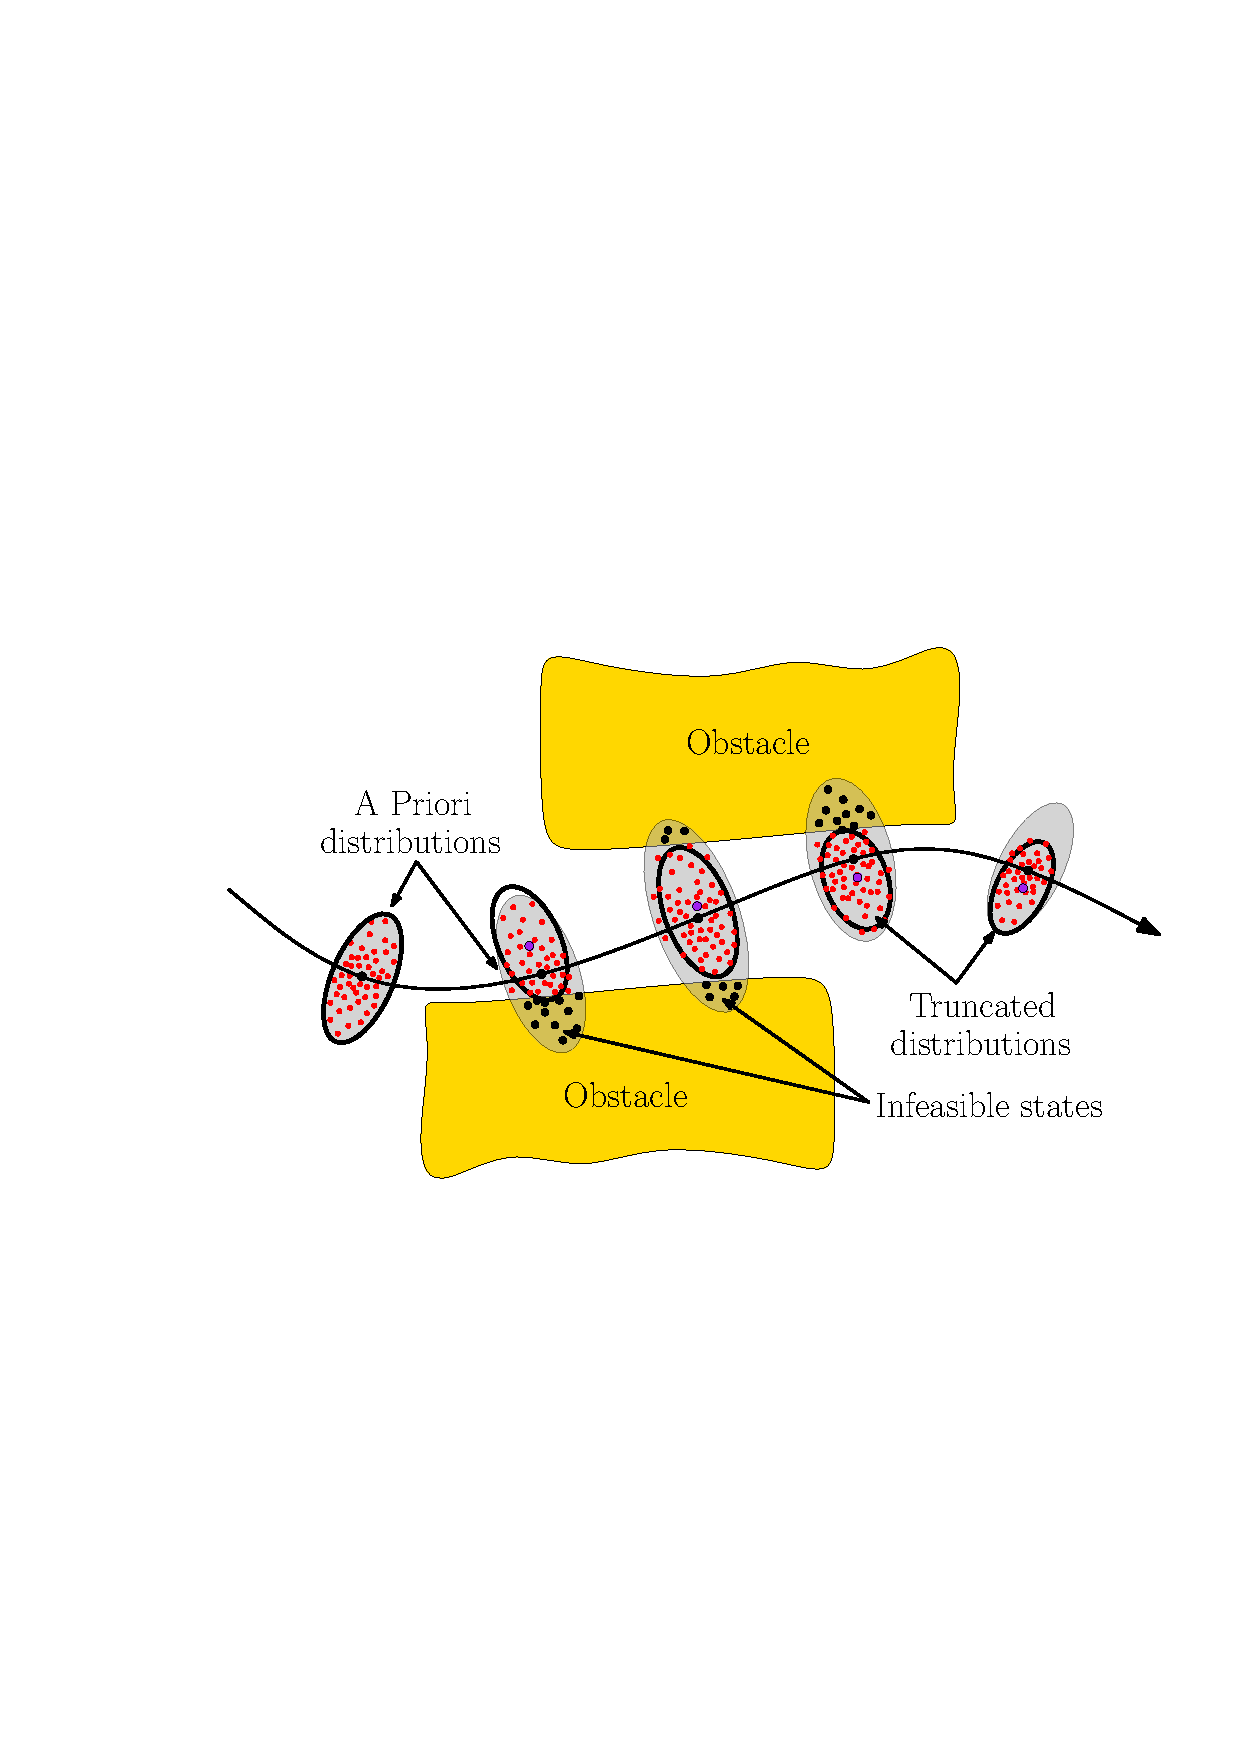
\includegraphics[width=240pt,clip]{figures/truncatedGaussians3.pdf}
\vspace{-5pt}
\caption{We estimate the probability of collision based on a priori probability distributions of the robot state. The probabilities of collision at each stage of the plan are conditioned on the previous stages being collision free. We propose a novel method to truncate the a priori distributions with respect to obstacles to discount plan executions that collide with obstacles (black disks). Propagating the truncated distributions (black ellipses) accounts for only the collision free samples (red disks), resulting in accurate estimation of the probability of collision. Approximating the collision probability based on the unconditional distributions (gray ellipses), as is done in most prior work, results in a very conservative estimate of the collision probability.}
\label{fig:teaser}
\vspace*{-10pt}
\end{figure}

In this work, we present a fast, analytical method that estimates the probability of collision for a robot executing a motion plan under the assumptions of Gaussian motion and sensing uncertainty. %We then demonstrate how this metric can be applied to a variety of existing motion planners to improve the safety and quality of the computed plans.
Formally speaking, let $\mathbf{x}_t \in \mathcal{X}$ denote the state of the robot at stage $t$ along the plan, and $\mathcal{X}_{F} \subset \mathcal{X}$ denote the feasible space not occupied by obstacles. The probability that a plan consisting of $\ell$ stages is collision free is then given by:
\begin{align}
p(\bigwedge_{t = 0}^{\ell}\; \mathbf{x}_t \in \mathcal{X}_{F}) = \prod_{t = 0}^\ell p(\mathbf{x}_{t} \in \mathcal{X}_{F}\; |\; \bigwedge_{i = 0}^{t-1} \; \mathbf{x}_i \in \mathcal{X}_{F}). \nonumber
\end{align}
Hence, to accurately estimate the probability of collision, we need to compute the distribution of the state at each stage along the plan \emph{conditioned} on the previous stages being collision free. This amounts to propagating the a priori distributions forward in time in such a way that instances that collide with obstacles are discounted from the propagation (Fig. \ref{fig:teaser}). For this we propose a novel method to truncate the a priori distributions with respect to obstacles, approximate the truncated distributions by Gaussians, and propagate them forward in time. This results in an accurate estimate of the conditional distributions, and consequently, enables accurate estimation of the collision probability.

Existing approaches, in contrast, typically ``approximate'' the collision probability of a plan by assuming the probabilities of collision at stages along the plan are independent, i.e., $p(\bigwedge_{t = 0}^{\ell} \; \mathbf{x}_t \in \mathcal{X}_{F}) \approx \prod_{t = 0}^\ell p(\mathbf{x}_{t} \in \mathcal{X}_{F})$ \cite{vandenBerg11_IJRR, Vitus11_ICRA, Bry11_ICRA}. This yields an overly conservative estimate of the probability of collision (see Fig.\ \ref{fig:teaser}), which might result in overly conservative motion plans and, depending on the safety required by the motion planner, may result in failure to find a feasible plan even if one exists.


%\begin{align}
%P(\bigcap\limits_{t = 0}^{\ell} \mathbf{x}_t \in \mathcal{X}_{F}) = \prod_{t = 0}^\ell P(\mathbf{x}_{t} \in \mathcal{X}_{F} | \bigcap\limits_{i = 0}^{t-1} \mathbf{x}_i \in \mathcal{X}_{F}) %\nonumber.
%\end{align}

%\begin{align}
%P(\bigcap\limits_{t = 0}^{\ell} \mathbf{x}_t \in \mathcal{X}_{F}) \approx \prod_{t = 0}^\ell P(\mathbf{x}_{t} \in \mathcal{X}_{F}) \nonumber,
%\end{align}

%The key insight in our method is that, unlike prior methods, we should not double-count the effect of collisions when estimating the a priori probability of collision of a plan.
%Truncating these distributions effectively discounts all plans that would potentially collide with obstacles during execution.

% TODO: This point should be made in section 4
%Even though the exposition outlines a method to truncate the distributions with respect to obstacles, we can directly apply this methodology to estimate the a a priori distributions with other constraints on the state variables (such as imposing limits on velocity, acceleration etc. of the robot).
Our method can either be directly used to quantify the safety of a plan \cite{vandenBerg11_IJRR, Patil11_RSS}, to accurately estimate collision chance constraints \cite{Bry11_ICRA, Vitus11_ICRA}, or to elegantly account for hard state constraints imposed by obstacles in optimization based \cite{Platt10_RSS, Erez10_UAI, vandenBerg11_ISRR} or inference based \cite{Toussaint09_ICML} planning methods. Our truncation approach is also directly applicable to the important problem of optimal state estimation with hard state constraints \cite{Book:Simon06}.

We present simulation results for a car-like robot with second-order dynamics, and a nonholonomic bevel-tip flexible needle, navigating with stochastic dynamics while operating under the guidance of partial and noisy state measurements. Our results suggest that our method is orders of magnitude faster than na\"{i}ve sampling based methods, and the mean error in estimating the probability of collision is considerably lesser as compared to prior methods.
